\documentclass[useAMS,usenatbib]{mn2e}
\pdfminorversion=4

% The following is needed to fix the margins if using Letter-size paper
% REMOVE if your LaTeX uses A4 paper by default
\addtolength\topmargin{-1.8cm}
\usepackage{newtxtext}
\usepackage[varg]{newtxmath}

\usepackage{graphicx}
\usepackage{siunitx}
\bibliographystyle{mn2e}
\usepackage{astrojournals}
\usepackage{fixltx2e}

\begin{document}

\newcounter{ion}
\newcommand\fakesc[1]{\protect\scalebox{1.0}[0.8]{#1}}
\newcommand\ION[2]{\ensuremath{\mathrm{#1\,\fakesc{#2}}}}
\newcommand\ion[2]{\setcounter{ion}{#2}\ION{#1}{\Roman{ion}}}
\newcommand\hii{\ion{H}{2}}
\newcommand\oiii{[\ion{O}{3}]}
\newcommand\nii{[\ion{N}{2}]}
\newcommand\sii{[\ion{S}{2}]}
\newcommand\siii{[\ion{S}{3}]}
\newcommand\ha{\ensuremath{\mathrm{H\alpha}}}
\newcommand\kms{\ensuremath{\mathrm{km\ s^{-1}}}}
\newcommand\los{\ensuremath{_{\mathrm{los}}}}
\newcommand\pos{\ensuremath{_{\mathrm{pos}}}}
\newcommand\obs{\ensuremath{_{\mathrm{obs}}}}
\newcommand\ins{\ensuremath{_{\mathrm{ins}}}}
\newcommand\rms{\ensuremath{_{\mathrm{rms}}}}
\newcommand\FS{\ensuremath{_{\mathrm{fs}}}}
\newcommand\therm{\ensuremath{_{\mathrm{therm}}}}
\addtocounter{section}{2}
\section{Results}
\addtocounter{subsection}{2}
\subsection{Plane-of-sky versus line-of-sight velocity variations}
\label{sec:plane-sky-versus}

 

\begin{figure}
  \centering
  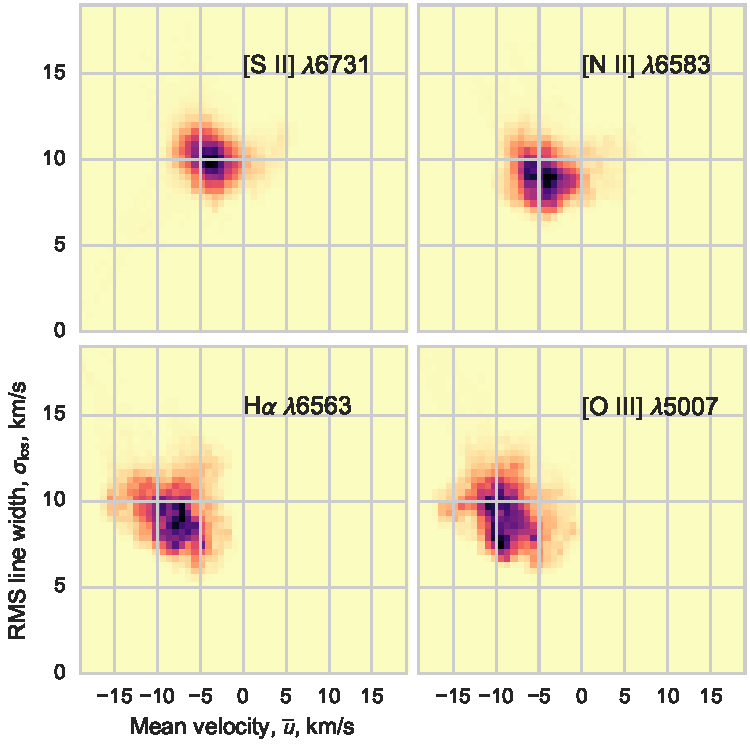
\includegraphics[width=\linewidth]{obs-combo-hist-vmean-sig}
  \caption{Joint distribution of moment-derived line-of-sight velocity
    dispersion and mean velocity.  The thermal, instrumental, and
    fine-structure contributions to the velocity dispersion have been
    subtracted in quadrature.  Mean velocities are shown with respect
    to the systemic velocity of the stellar cluster (\(+7~\kms\) in
    the Local Standard of Rest frame, or \(+25~\kms\) in the
    Heliocentric frame, \citealp{Tobin:2009a}).}
  \label{fig:observed-vmean-sigma}
\end{figure}
The non-thermal line-of-sight velocity dispersion 
\(\sigma\los\)
may be estimated by
correcting the observed line widths for the contributions from the
spectrograph resolution, %\(\sigma\ins \approx \SI{3.4}{km s^{-1}} \),
fine-structure splitting, %\(\sigma\FS\), 
and thermal Doppler broadening, 
% \(\sigma\therm \approx 9.1 (T_4 / A)^{1/2} \ \si{km
%   s^{-1}}\), where \(T_4 = T / \SI{e4}{K}\) and \(A\) is the atomic
% weight.  
as in Eq.~(2) of \citet{Garcia-Diaz:2008a}.  
% \begin{equation}
%   \label{eq:1}
%   \sigma\los^2 = \sigma\obs^2 - \sigma\ins^2 - \sigma\FS^2 - \sigma\therm^2
% \end{equation}
A striking fact about the nebular line profiles is that
the line-of-sight velocity dispersion is several times larger than the
plane-of-sky dispersion in mean velocities.  This is illustrated in
Figure~\ref{fig:observed-vmean-sigma}, which shows flux-weighted
histograms of the non-thermal RMS line widths versus mean velocity for
all lines of the \citet{Garcia-Diaz:2008a} spectral axis.   The
line-of-sight RMS velocity dispersion is 9--10~\kms, whereas the RMS
plane-of-sky dispersion of the mean velocities is only 2--4~\kms.  
% In the case of \ha{} and \oiii{}

\begin{figure}
  \centering
  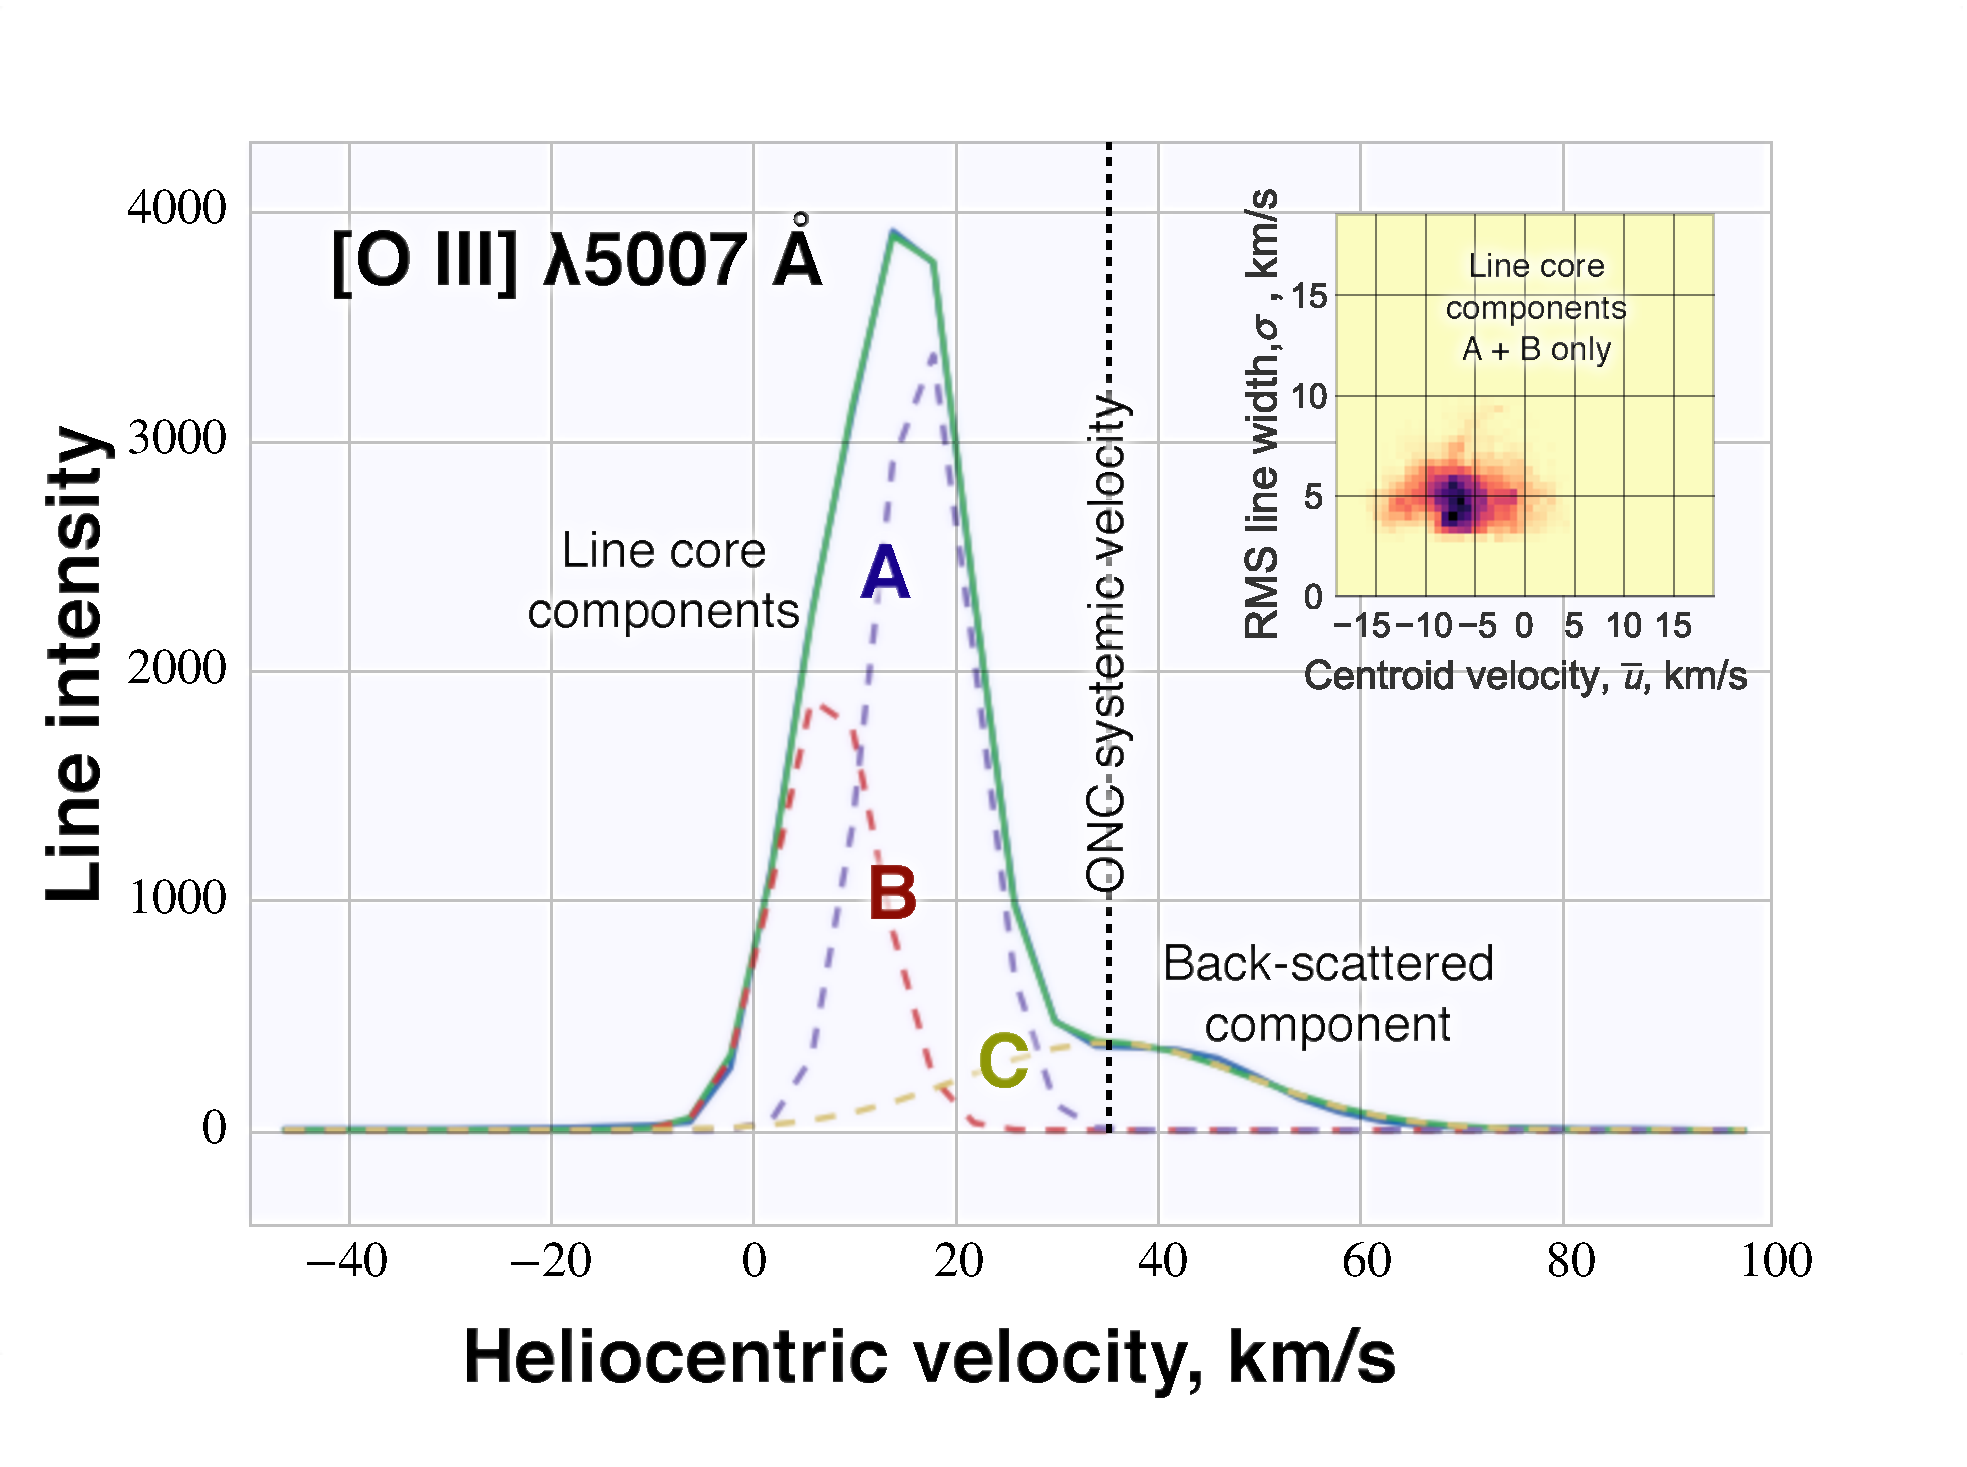
\includegraphics[width=\linewidth]{ABC-profile-example}
  \caption{Typical [\ion{O}{3}] line proile, showing Gaussian
    decomposition into three components, following the labeling of
    \citet{Castaneda:1988a}.  The red-shifted component~C is due to
    back-scattering of the blue-shifted components A and B by dust
    that lies behind the emitting gas.  Inset figure is same as
    Fig.~\ref{fig:observed-vmean-sigma}, but after removing
    Component~C from the profile.}
  \label{fig:gauss}
\end{figure}

However, the observed line widths are affected by additional
broadening due to dust-scattering \citep{Castaneda:1988a,
  Henney:1998a}, which gives an extended red
wing to the line profile that contains 10--20\% of the total line
flux (see Fig.~\ref{fig:gauss}).   By means of fitting multiple
Gaussian components to each line profile, it is possible to
effectively remove this scattered component and calculate statistics
for the line core alone.  We have done this for the \oiii{} line, with
results shown in the inset box of Figure~\ref{fig:gauss}.  It can be
seen that the line-of-sight velocity dispersion is reduced by almost a
factor of two.  

\begin{figure}
  \centering
  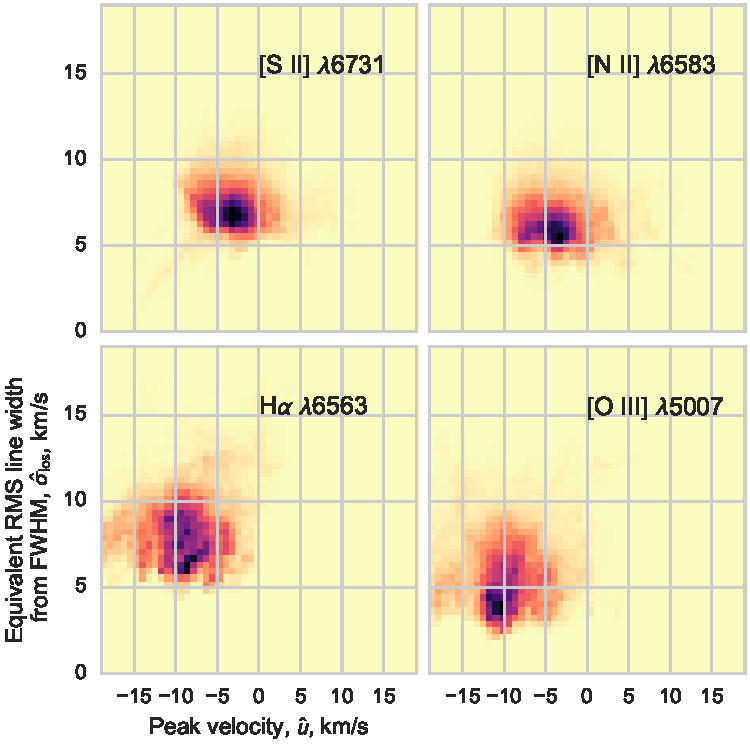
\includegraphics[width=\linewidth]{obs-combo-hist-vpeak-fwhm.pdf}
  \caption[]{Same as Fig.~\ref{fig:observed-vmean-sigma} but
    substituting the FWHM-derived line width \(\hat{\sigma}\los\) for the
    moment-derived line width \(\sigma\los\) and substituting the peak
    velocity \(\hat{u}\) for the mean velocity \(\bar{u}\).  }
  \label{fig:observed-vmean-sigma-fwhm}
\end{figure}

It is more difficult to perform the Gaussian decomposition for the
lower ionization lines since the back-scattered component is not as
cleanly separated from the core component.  On the other hand, an
alternative method of suppressing the effects of scattering on the
line widths is to use the Full Width at Half Maximum (FWHM) instead of
the RMS width.  Even a weak component with a velocity that is very
different from the line centroid can have a large effect on the
\(\sigma\los\) due to the \((u - \bar{u})^2\) dependence of the second
velocity moment.  But the same component will have almost no effect on
the FWHM if its amplitude is less than half that of the line core.  We
therefore define a FWHM-based effective \(\sigma\) as
\(\hat{\sigma}\los = \mathrm{FWHM} / \sqrt{8 \ln 2} \approx
\mathrm{FWHM} / 2.355\), with the constant of proportionality being
chosen so that \(\hat{\sigma}\los = \sigma\los\) for a Gaussian profile.  The
results are shown in Figure~\ref{fig:observed-vmean-sigma-fwhm}, where
it can be seen that nearly all the lines show substantial reductions
in the line-of-sight line widths with respect to the moment-derived
values of Figure~\ref{fig:observed-vmean-sigma}.  The exception is
\ha{}, where larger thermal broadening means that \(\hat{\sigma}\los\) is
still contaminated by the back-scattered component due to blending.
Note that \(\hat{\sigma}\los\) is insensitive to not only the scattered
component, but also to any other weak component that is not blended
with the line core.  For the low-ionization lines such as \nii{} and
\sii{}, this includes the kinematic component known as the Diffuse
Blue Layer \citep{Deharveng:1973a}, which produces line splitting in
the SE and N regions of our observed maps.  


\begin{figure}
  \centering
  \begin{tabular}{@{}l@{}l@{}}
    (\textit{a}) & (\textit{b}) \\
    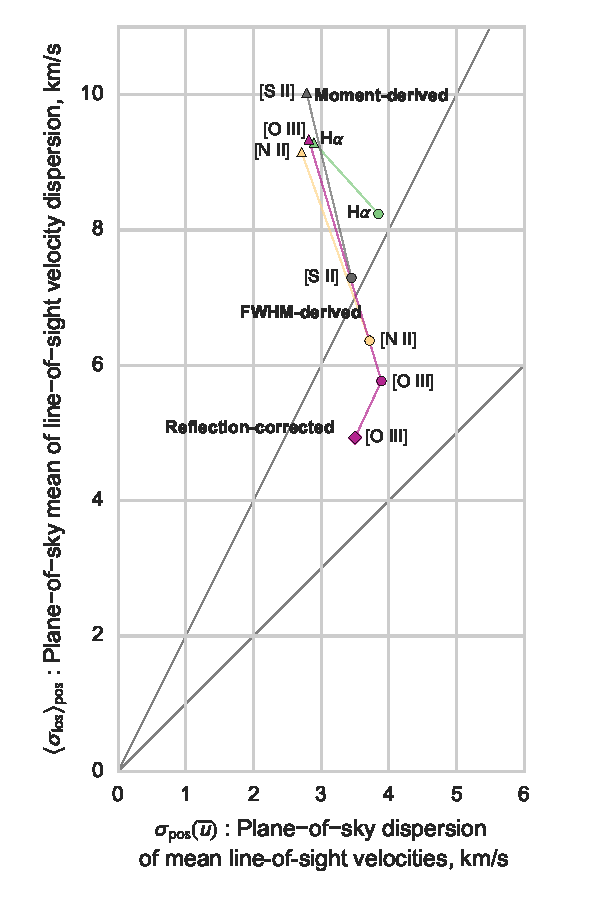
\includegraphics[width=0.48\linewidth]{obs-stats-plot} 
    & 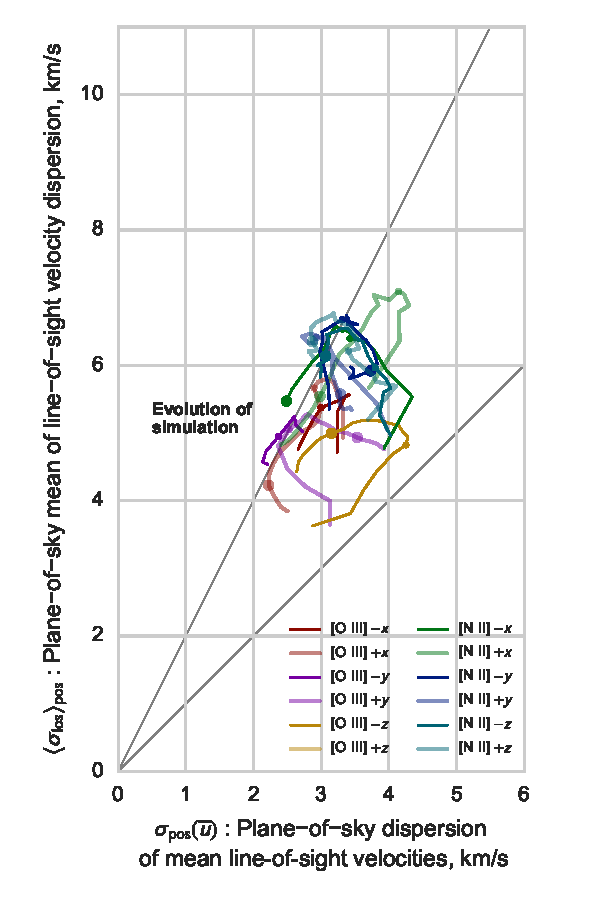
\includegraphics[width=0.48\linewidth]{sim-stats-plot} \\
  \end{tabular}
  \caption{(\textit{a})~Observational comparison of mean line-of-sight
    velocity dispersion (vertical axis) with plane-of-sky dispersion
    of mean line-of-sight velocity (horizontal axis).  All averages
    were performed with flux weighting.  Triangle symbols show the
    moment-derived values, which are contaminated by the
    back-scattered component.  Circle symbols show the more robust
    FWHM-derived values, while the diamond symbol shows the
    reflection-corrected result from multi-Gaussian fitting, which was
    only possible for \oiii.  The diagonal white lines show the
    relationships \(\sigma\los = \sigma\pos\) and \(\sigma\los =
    2\sigma\pos\).  (\textit{b})~The same quantities derived
    from evolutionary tracks of the turbulent \hii{} region simulation
    described in \citet{Medina:2014a} for different viewing directions
    as shown in the key: blue/green lines are for \nii{}, while
    red/purple/yellow lines are for \oiii{}. Evolutionary times of
    0.15~Myr (small dot) and 0.25~Myr (larger dot) are marked on each
    track, and only those times where the mean line velocity is
    blueshifted are shown.  }
  \label{fig:obs-sigma-sigma}
\end{figure}

\section{Discussion}
\addtocounter{subsection}{2}
\subsection{Turbulent contribution to spectral line broadening}
\label{sec:turb-contr-spectr}
So far we have concentrated on the slopes of the structure function
and power spectra, since they can be theoretically related to the
spectrum of underlying velocity fluctuations in the nebula.  However,
other questions require consideration of the magnitude of the velocity
fluctuations, as measured by different techniques.  Such questions
include whether turbulence alone is sufficient to account for the non-thermal
line broadening observed in the nebula, and whether that turbulence is
driven primarily by the large scale thermal expansion of the nebula,
or by smaller scale photoevaporation flows, and to what extent stellar
winds play a role. 

The plane-of-sky dispersion in centroid velocities
\(\sigma\pos(\bar{u})\) is the RMS width of the marginal distribution
along the \(\bar{u}\) axis of Figure~\ref{fig:observed-vmean-sigma},
which is the same as the quantity \(\sigma_{\mathrm{vc}}\) used to
normalize the structure functions in \S~2.
Figure~\ref{fig:obs-sigma-sigma}(\textit{a}) summarizes the
observational determination of \(\sigma\los\) and \(\sigma\pos\),
while Figure~\ref{fig:obs-sigma-sigma}(\textit{b}) shows the same
quantities calculated for the turbulent \hii{} region simulation of
\citet{Medina:2014a}, as presented in the Appendix.  As discussed in
\S~\ref{sec:plane-sky-versus}, the FWHM-derived and
reflection-corrected observational values are the most reliable, and
these fall broadly in the same region of the graph as do the
evolutionary tracks, with \(\sigma\pos \approx 3 \pm 1 \ \kms\) and
\(\sigma\los \approx 6 \pm 1 \ \kms\).

The fact that the line-of-sight velocity dispersion is roughly twice
the plane-of-sky velocity dispersion can be interpreted in at least
two different ways.  In the case of a homogeneous turbulent velocity
field with characteristic correlation length \(l_0\), the projection
from three to two dimensions over a line-of-sight depth \(L\) reduces
the plane-of-sky amplitude of fluctuations if \(l_0 < L\), a
phenomenon known as ``projection smearing'' \citep{von-Hoerner:1951a,
  Scalo:1984a}.  Our \(l_0\) and \(\sigma\pos / \sigma\los\)
correspond to \(s_0\) and
\(\sigma_{\mathrm{obs}} / \sigma_{\mathrm{true}}\) in Fig.~1 of
\citet{Scalo:1984a}, from which it can be seen that a value of \(0.5\)
requires \(l_0 / L \approx 0.02\)--\(0.1\), depending on the steepness
of the velocity fluctuation spectrum.  The results from our structure
function analysis (\S~\ref{subsec:sf}) imply a correlation length
\(l_0 \approx 0.1\)--\(0.2\)~pc for all lines, which would require a
very large line-of-sight depth \(L > 1\)~pc in order to explain the
observed \(\sigma\pos / \sigma\los\) by projection smoothing.  This is
wildly inconsistent with independent evidence \citep{Baldwin:1991a,
  ODell:2001b, Garcia-Diaz:2007a} that the emitting layer thickness is
much smaller than this in the region covered by our maps:
\(L \approx 0.01\)--\(0.3\)~pc, being thinner on the West side and for
the lower ionization lines.

The same discrepancy arises when the projection smearing argument is
applied to our simulated \hii{} region.  In this case,
\(l_0 \approx 0.5\)--\(1\)~pc for evolutionary times later than
\(0.15\)~Myr (Fig.~A4 of \citealp{Medina:2014a}), thus requiring
\(L > 5\)~pc, which is clearly unacceptable since it is bigger than the
computational box of the simulation.  For both the simulation and the
observations, it is clear that \(l_0 \approx L\) for the
high-ionization lines and \(l_0 > L\) for the low-ionization lines.
Therefore, projection smearing of the large-scale fluctuations is
negligible and cannot explain the difference between \(\sigma\pos\)
and \(\sigma\los\). 

\begin{figure}
  \centering
  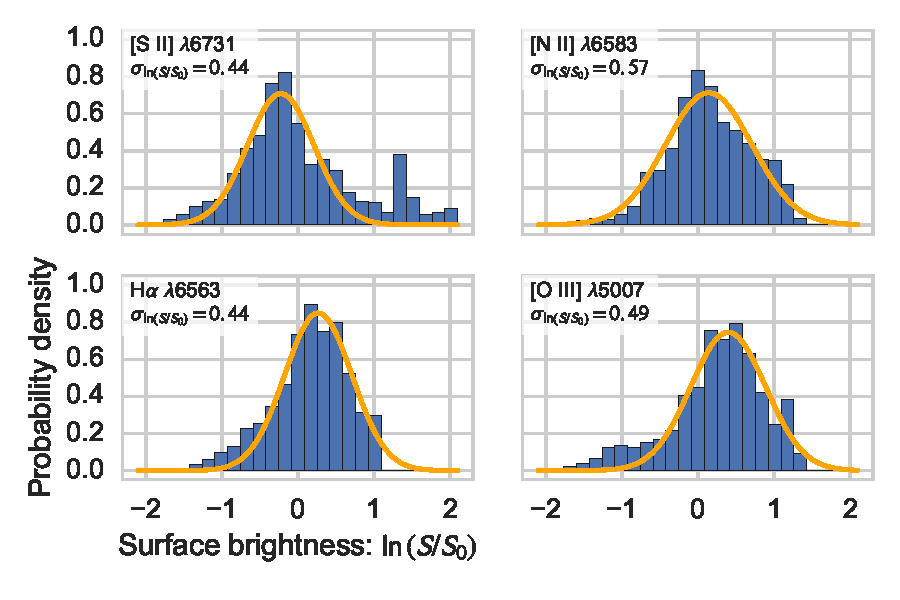
\includegraphics[width=\linewidth]{bright-hist-obs}
  \caption{Probability density functions (PDF, blue histograms) of
    observed surface brightness maps in different emission lines after
    binning \(16 \times 16\) pixels to eliminate small scale
    variations.  The surface brightness is normalized by the mean
    value and shown on a natural logarithmic scale, and the PDFs are
    weighted by the surface brightness itself.  A log-normal
    distribution (orange lines) is fitted to the core of each PDF
    (only the part of the histogram with probability density \(> 0.3\)
    times the maximum).  The fitted RMS width \(\sigma\) of the
    log-normal distribution is indicated on each panel.}
  \label{fig:surf-bright-pdf}
\end{figure}

\newcommand\Efrac{\ensuremath{_{\scriptscriptstyle E/E_0}}}
\newcommand\lnSfrac{\ensuremath{_{\scriptscriptstyle \ln S/S_0}}}
\newcommand\Sfrac{\ensuremath{_{\scriptscriptstyle S/S_0}}}

A second, contrasting interpretation of the evidence would be in terms
of large-scale, ordered motions.  Consider an emission shell that
expands at velocity \(v\).  If the shell emissivity is homogeneous,
then the integrated line profile is rectangular, with mean velocity
\(\bar{u} = 0\) and velocity width \(\sigma\los = v/2\).  Furthermore,
the spatially resolved line profile at any point will also have
\(\bar{u} = 0\), so that \(\sigma\pos = 0\).  However, if there are
emissivity fluctuations between different parts of the shell, then
\(\bar{u}\) will fluctuate on the plane of the sky, according to the
relative brightness of the red-shifted and blue-shifted hemispheres.
The required RMS fractional variation in the emissivity on the scale
of the shell diameter is found to be \(\sigma\Efrac \approx
\sigma\pos/\sigma\los\). 

The observed large-scale (\(> 9''\)) brightness fluctuations are
illustrated in Figure~\ref{fig:surf-bright-pdf}, which shows
log-normal fits to the PDFs of surface brightness, \(S\), after
normalizing by the mean, \(S_0\), and binning the maps at
\(16 \times 16\) pixels.  The RMS width of the log-normal PDF,
\(\sigma\lnSfrac\) is seen to be in the range 0.45--0.6 for all lines.
This is related to the RMS fractional brightness fluctuation as
\(\sigma^2\lnSfrac = \ln(1 + \sigma^2\Sfrac)\), or
\(\sigma\lnSfrac \approx \sigma\Sfrac\) if \(\sigma\Sfrac < 1\).  The
relationship between \(\sigma\Efrac\) and \(\sigma\Sfrac\) depends on
both line-of-sight projection \citep{Brunt:2010b}, which tends to make
\(\sigma\Sfrac < \sigma\Efrac\), and fluctuations in the foreground
dust extinction, which have the opposite effect of increasing
\(\sigma\Sfrac\).  We assume that the two effects roughly cancel, so
that the surface brightness PDFs imply
\(\sigma\Efrac \approx \sigma\Sfrac \approx 0.5\).  This is equal to
the value derived in the previous paragraph to be required by the
observed \(\sigma\pos/\sigma\los\), which implies that emissivity
fluctuations combined with an ordered velocity field are entirely
sufficient to explain the observed plane-of-sky variation in mean
velocities, without requiring any fluctuations in the velocity field
itself.

\newcommand\champ{\ensuremath{_{\mathrm{cham}}}}
\newcommand\turb{\ensuremath{_{\mathrm{turb}}}}
\newcommand\oi{[\ion{O}{1}]}
Although it is a priori unlikely that there are \textit{no} velocity
fluctuations in the ionized gas, this is yet another reason why the
structure function of the mean velocity is not an effective diagnostic
of these fluctuations in the presence of strongly inhomogeneous
emissivity and large-scale velocity gradients.  In Orion, the ordered
large scale expansion of the nebula is an asymmetrical champagne flow
away from the background molecular cloud \citep{Zuckerman:1973a}, which
produces systematically larger blue-shifts with increasing ionization
(e.g., Fig.~11 of \citealp{Baldwin:2000a}).  This offers a simple
method for estimating the relative contribution of ordered versus
turbulent motions to the total velocity dispersion.  The mean
systematic difference between the \oi{} and \oiii{} centroid
velocities is \(\delta u = 9.4~\kms\) (Table~2 of
\citealp{Garcia-Diaz:2008a}), which gives a champagne-flow
contribution to the velocity dispersion of \(\sigma\champ \approx 0.5\,
\delta u = 4.7~\kms\).   The turbulent contribution to the velocity
dispersion is then \(\sigma\turb \approx (\sigma\los^2 -
\sigma\champ^2)^{1/2} = 3.7~\kms\).  The uncertainties in this
analysis are large, so that all that can be confidently asserted is
that the ordered and turbulent velocity dispersions are roughly equal
with \(\sigma\champ \sim \sigma\turb = 4\)--\(5~\kms\).


\appendix

\section[]{\boldmath Plane-of-sky versus line-of-sight variations in velocity from
simulated \hii{} region}

\begin{figure}
  \centering
  \setkeys{Gin}{width=0.47\linewidth}
  \begin{tabular}{@{}ll@{}}
    (\textit{a}) & (\textit{b}) \\
    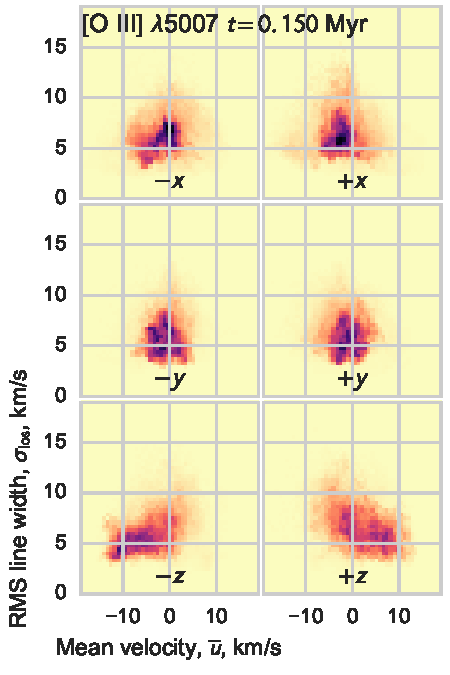
\includegraphics{hist-vmean-sig-0015-O35007}
    & 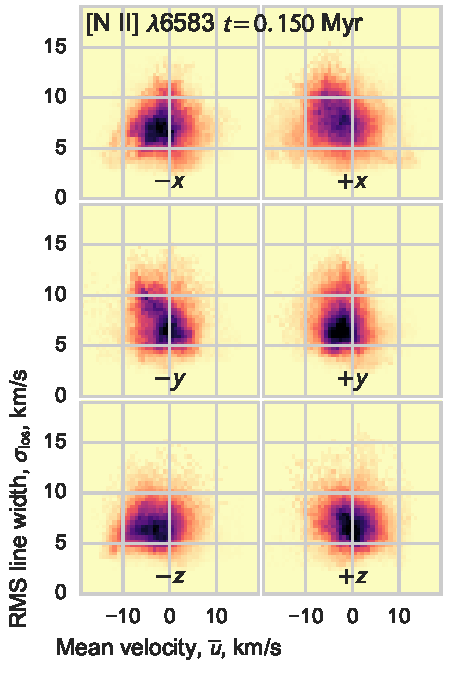
\includegraphics{hist-vmean-sig-0015-N26584}\\
    \\
    (\textit{c}) & (\textit{d}) \\
    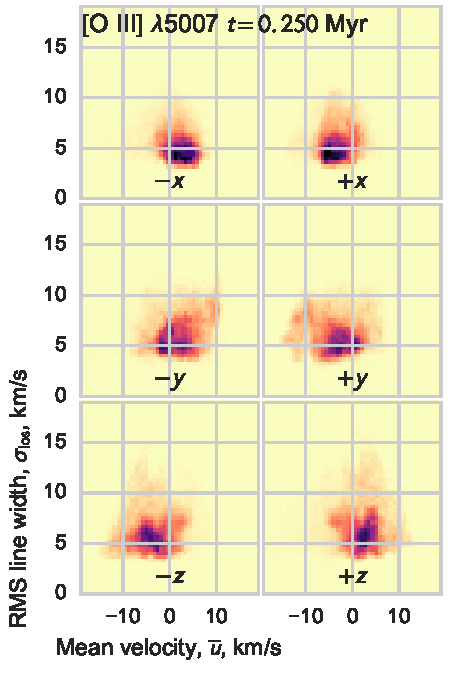
\includegraphics{hist-vmean-sig-0025-O35007}
    & 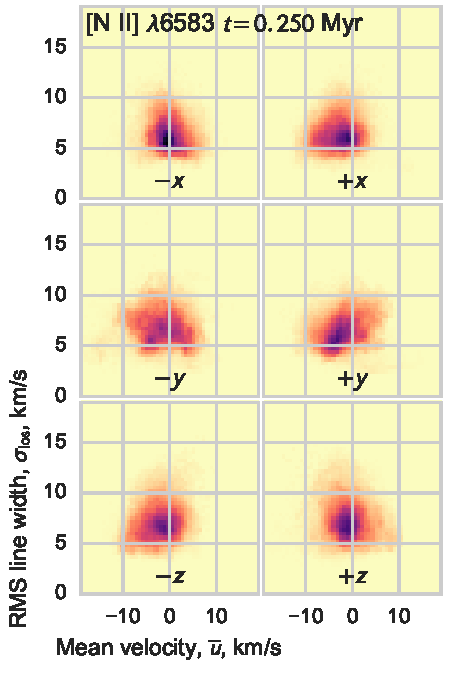
\includegraphics{hist-vmean-sig-0025-N26584}\\
  \end{tabular}
  \caption{Joint probability densities of mean velocity \(\bar{u}\)
    and line-of-sight velocity dispersion \(\sigma\los\) for two
    representative times in the evolution of a simulated \hii{}
    region: 0.15~Myr (\textit{a} and \textit{b}) and 0.25~Myr
    (\textit{c} and \textit{d}).  Line profile parameters are
    calculated for each position-position pixel of a synthetic
    position-position-velocity cube of the \oiii{} line (\textit{a}
    and \textit{c}) and \nii{} line (\textit{b} and \textit{d}), which
    takes into account dust absorption (but not scattering) and
    thermal broadening at the local temperature. In each subfigure,
    results are shown for six viewing directions that correspond to
    the positive and negative principal axes of the simulation cube.
    The average thermal velocity width is subtracted in quadrature in
    order to mimic the observational methodology for isolating the
    non-thermal contribution to \(\sigma\los\). }
  \label{fig:simulation-vmean-sigma}
\end{figure}

\begin{figure}
  \centering
  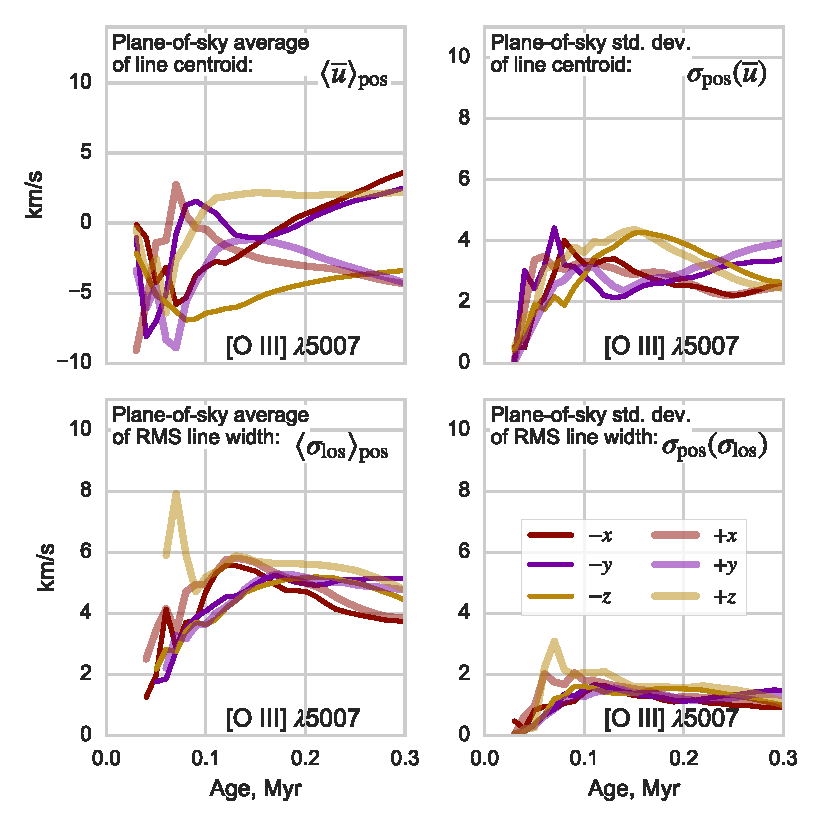
\includegraphics[width=\linewidth]{pos-stats-evo-O35007}
  \caption{Temporal evolution of velocity statistics calculated from
    synthetic observed position-position-velocity cubes of the \oiii{}
    line, as illustrated in left panels of
    Fig.~\ref{fig:simulation-stats-evo}.  Top row shows plane-of-sky
    average (left) and standard deviation (right) of the mean line
    velocity \(\bar{u}\), while bottom row shows the same for the
    non-thermal RMS line width \(\sigma\los\).  Different colored
    lines correspond to viewing directions along each of the cube
    axes.}
  \label{fig:simulation-stats-evo}
\end{figure}


For two representative times, Figure~\ref{fig:simulation-vmean-sigma}
shows the joint distribution of mean velocity \(\bar{u}\) and
non-thermal line width \(\sigma\los\), calculated from the line
profiles of synthetic position-position-velocity cubes for the
simulated turbulent \hii{} region of \citet{Medina:2014a}.
Figure~\ref{fig:simulation-stats-evo} shows the temporal evolution of
the plane-of-sky average and standard deviation of the same two
quantities for the \oiii{} line.  Results from the upper-right and
lower-left panel of Figure~\ref{fig:simulation-stats-evo} respectively
provide the data that go into the horizontal and vertical axes of
Figure~\ref{fig:obs-sigma-sigma}(\textit{b}) in
\S~\ref{sec:turb-contr-spectr}.

At late times (Fig.~\ref{fig:simulation-vmean-sigma}\textit{c,d}),
when dust absorption is relatively unimportant, the average line
centroid velocity (upper left panel of
Fig.~\ref{fig:simulation-stats-evo}) reflects the champagne flow due
to the largest-scale density gradients in our simulation box.  This
leads to both blue and red shifts, since opposite viewing directions
(e.g., \(+x\) and \(-x\)) have roughly equal but opposite mean
velocities, so that pairs of PDFs in
Fig.~\ref{fig:simulation-vmean-sigma}\textit{c,d} are rough mirror
images.  At earlier times
(Fig.~\ref{fig:simulation-vmean-sigma}\textit{a,b}), radial expansion
dominates and the dust optical depth is larger, which leads to
selectively greater absorption of receding regions of the nebula.
This produces predominantly blue-shifted mean velocities from all
viewing directions.


\bibliography{BibdeskLibrary-slavoj}

\end{document}

%%% Local Variables:
%%% mode: latex
%%% TeX-master: t
%%% End:
